% ============================================================
%  Metodología y desarrollo
% ============================================================
\section{Metodología y desarrollo}
\label{sec:metodologia}

El desarrollo siguió una estrategia incremental: primero se definieron los
criterios de ensayo a partir de la norma, luego se construyeron por separado el
dispositivo y la interfaz, y finalmente se integraron y verificaron en un banco de
pruebas real con cargas conocidas. Esta sección describe el diseño del hardware,
el del software y los criterios metodológicos adoptados para cada ensayo.

% ------------------------------------------------------------
\subsection{Desarrollo del hardware}
\label{subsec:metodologia_hw}
% ------------------------------------------------------------

\subsubsection{Equipo completo de referencia y prototipo propio}
\label{subsubsec:equipo_syglab}

El trabajo se apoyó en dos equipos con propósitos distintos:
\begin{itemize}
    \item \textbf{Equipo completo de referencia:} un equipo de ensayos de final de
          línea provisto por SYGlab, que realiza los ensayos de consumo,
          corriente de fuga, puesta a tierra, tensión resistida (rigidez
          dieléctrica) y corte de neutro, con la misma
          arquitectura de este proyecto: medidores PZEM, relés, contactores y
          transformadores de ensayo comandados desde una PC. El hardware fue
          provisto por SYGlab; su esquematización ---el relevamiento del
          conexionado y los esquemas de conexión de cada ensayo
          (Anexo~\ref{anx:evidencia})--- fue realizada por la autora. En ese equipo
          se ejecutó la versión inicial del software desarrollado en este
          trabajo, que luego se amplió y corrigió hasta su versión final.
    \item \textbf{Prototipo propio:} un banco armado por la autora para el ensayo
          de consumo, sobre el que se desarrolló y verificó de punta a punta la
          versión final del software con hardware real
          (Figura~\ref{fig:conexion_red}).
\end{itemize}

\subsubsection{Criterios de selección de componentes}

La selección de los componentes se realizó mediante un análisis de mercado con
los siguientes criterios:
\begin{enumerate}
    \item \textbf{Relación calidad-precio:} componentes con prestaciones adecuadas
          para los rangos de medición de la norma, sin recurrir a equipamiento
          industrial de alta gama.
    \item \textbf{Soporte y documentación:} plataformas con documentación técnica,
          bibliotecas activas y comunidades consolidadas, lo que reduce el riesgo
          de obsolescencia y facilita la resolución de problemas.
    \item \textbf{Disponibilidad:} componentes presentes en distribuidores
          nacionales y en plataformas de importación, para asegurar la reposición.
\end{enumerate}

\subsubsection{Componentes del dispositivo}

\paragraph{Unidad de procesamiento --- ESP32.}
Se utiliza un módulo de desarrollo ESP32 NodeMCU-32S (Espressif), con conversor
USB-serie CP2102. Es un sistema en chip de doble núcleo a \SI{240}{\mega\hertz}
con varios puertos UART, lo que permite atender a la PC por USB y, a la vez, a los
medidores por un segundo puerto serie. Su conectividad inalámbrica deja abierta la
comunicación remota en versiones futuras sin hardware adicional.

\paragraph{Medidores --- PZEM-004T.}
La adquisición de parámetros eléctricos se realiza con módulos PZEM-004T
(Peacefair) \cite{pzem004t}, que miden tensión (resolución \SI{0,1}{\volt}),
corriente (resolución \SI{0,001}{\ampere}), potencia activa (resolución
\SI{0,1}{\watt}), energía, frecuencia y factor de potencia, con una exactitud
declarada de \SI{0,5}{\percent}. La arquitectura prevé tres módulos: PZEM1 para
consumo, PZEM2 para fuga y rigidez dieléctrica y PZEM3 para puesta a tierra. En
el banco se utilizó la versión~4.0 de \SI{100}{\ampere} con transformador de
corriente toroidal, adecuada para el ensayo de consumo. Esta versión no resuelve
las corrientes de fuga (su umbral de arranque es del orden de
\SI{20}{\milli\ampere}, frente a un límite de \SI{0,75}{\milli\ampere}), por lo
que el ensayo de fuga requiere la versión de \SI{10}{\ampere} con derivador
(\emph{shunt}) y una red de medición según IEC~60990 \cite{iec60990}.

\paragraph{Conmutación --- contactores y relés.}
La tensión de red hacia el DUT y hacia cada circuito de ensayo se conmuta con
contactores con bobina de \SI{220}{\volt}, cuya apertura mecánica asegura la
separación entre etapas. En el banco se empleó un contactor CHINT NXC-12M/22
(2~NA + 2~NC, AC-1 \SI{20}{\ampere}, AC-3 \SI{12}{\ampere}) con un varistor
ZOV~10D431K entre los bornes de la bobina. Las bobinas se comandan desde la PC
mediante una placa de relés USB: el diseño final prevé un módulo HW-554 de ocho
canales y en el banco se utilizó una placa USB HID de dos canales.

\paragraph{Transformadores de ensayo.}
El equipo incorpora dos transformadores específicos:
\begin{itemize}
    \item \textbf{Rigidez dieléctrica}, elevador con salida seleccionable de
          \SI{1000}{\volt} (aislamiento básico, Clase~I) o \SI{2500}{\volt}
          (aislamiento reforzado, Clase~II) y corriente limitada a
          \SI{30}{\milli\ampere}. Esa limitación es una protección de la fuente,
          que acota la energía ante una ruptura del aislamiento, y no un límite de
          aprobación: el criterio de la norma es que la corriente no supere
          \SI{5}{\milli\ampere}, valor que puede elevarse hasta
          \SI{30}{\milli\ampere} en aparatos con alta corriente de fuga
          (Anexo~A.2).
    \item \textbf{Puesta a tierra}, reductor de \SI{2,2}{\volt} y
          \SI{75}{\volt\ampere}, previsto para entregar unos \SI{15}{\ampere}. La
          norma exige una corriente de al menos \SI{10}{\ampere} desde una fuente
          de no más de \SI{12}{\volt} (Anexo~A.1); que el transformador alcance esa
          corriente con el cableado real queda por verificar.
\end{itemize}

\paragraph{Protecciones.}
El banco incorpora fusibles de \SI{1}{\ampere} en la alimentación del medidor y de
la bobina del contactor, un fusible de \SI{10}{\ampere} en el camino del DUT y la
tierra de protección conectada directamente al DUT, sin pasar por el contactor.
El banco no cuenta con interruptor diferencial; el riesgo se mitiga por
procedimiento (no manipular nada energizado y desconectar antes de intervenir).

\paragraph{Instrumento patrón previsto.}
Para calibrar y validar metrológicamente el equipo se prevé contrastarlo con
instrumentos de exactitud claramente superior a la de los medidores PZEM, con
certificado de calibración trazable emitido por un laboratorio acreditado por el
OAA:
\begin{itemize}
    \item \textbf{Consumo:} un analizador de potencia de laboratorio, como el
          Yokogawa WT310E \cite{wt310e}, conectado en serie con el aparato para
          comparar ambas lecturas sobre la misma carga. Su exactitud en potencia
          es del orden de \SIrange{0,1}{0,15}{\percent}, entre tres y cinco veces
          mejor que el \SI{0,5}{\percent} del PZEM-004T.
    \item \textbf{Ensayos de seguridad:} un calibrador de equipos de ensayo de
          seguridad eléctrica, como el Fluke 5322A \cite{fluke5322a}. A
          diferencia de un segundo equipo de ensayo, el calibrador genera
          valores conocidos que el sistema debe medir: simula corrientes de fuga
          de \SIrange{0,1}{30}{\milli\ampere} con resolución de
          \SI{10}{\micro\ampere} (cubre el límite de \SI{0,75}{\milli\ampere}),
          ofrece resistencias de tierra a cuatro hilos desde
          \SI{1}{\milli\ohm} (cubre los límites de \SI{100}{\milli\ohm} y
          \SI{200}{\milli\ohm}) y mide la tensión de rigidez dieléctrica con un
          divisor de \SI{10}{\kilo\volt}.
\end{itemize}
Los patrones de resistencia y de fuga del modo de verificación se contrastarían
con el mismo calibrador antes de usarlos en producción.
Al cierre del trabajo este contraste no se había realizado
(Sección~\ref{sec:resultados}).

\paragraph{Carcasa.}
El equipo final se aloja en una valija de aluminio reforzada, del tipo
\emph{flight case}, con cierre por pestillos, manija y posibilidad de montar
paneles y riel DIN.

\subsubsection{Arquitectura del dispositivo}

El dispositivo se organiza en cinco bloques funcionales:
\begin{enumerate}
    \item \textbf{Potencia:} transformadores, contactores y protecciones.
    \item \textbf{Adquisición:} medidores PZEM-004T.
    \item \textbf{Control:} ESP32 y placa de relés USB.
    \item \textbf{Comunicación:} enlaces USB entre la PC, el ESP32 y la placa de
          relés.
    \item \textbf{Seguridad:} fusibles, tierra de protección, indicadores y paro de
          emergencia.
\end{enumerate}

\begin{figure}[htbp]
    \centering
    \figuraopcional{arquitectura_dispositivo.png}{0.85\linewidth}
    \caption{Diagrama general del dispositivo.}
    \label{fig:arquitectura_dispositivo}
\end{figure}

La Figura~\ref{fig:conexion_red} muestra la conexión de red, las protecciones y el
control del banco de pruebas construido. El esquema de cableado original y su
versión ilustrada se incluyen en el Anexo~\ref{anx:evidencia}.

\begin{figure}[htbp]
    \centering
    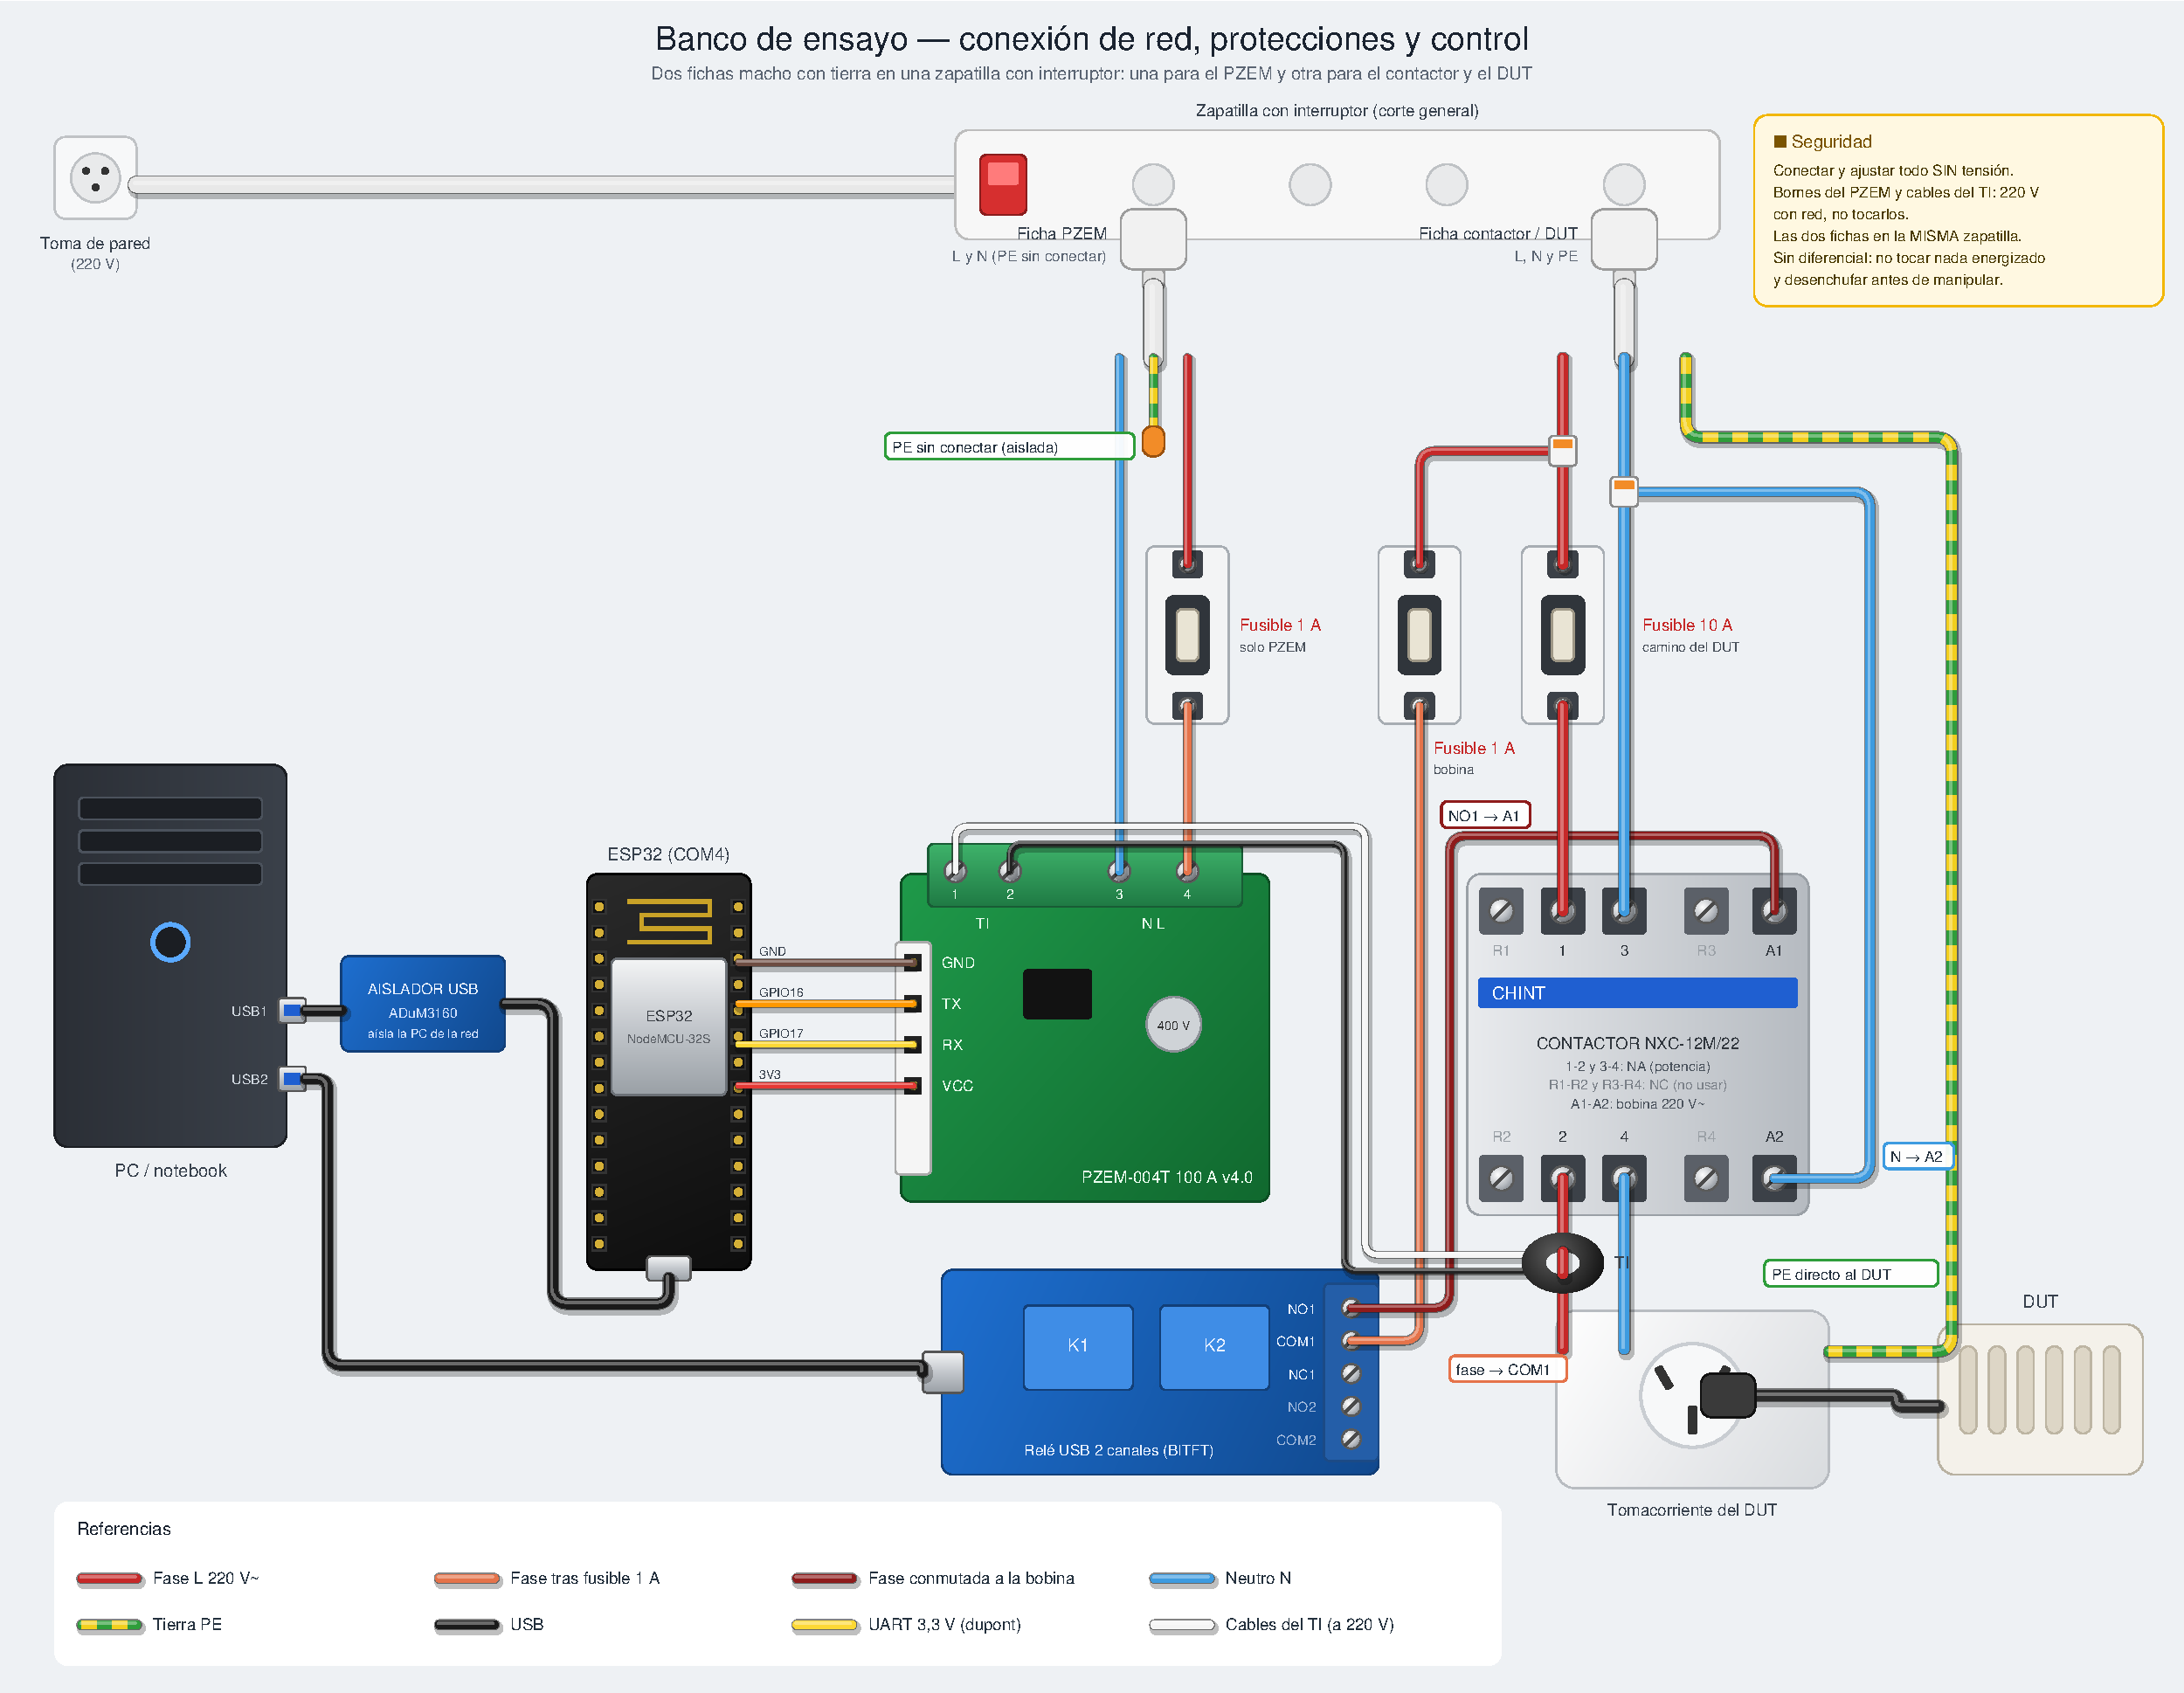
\includegraphics[width=\linewidth]{conexion_red_banco.pdf}
    \caption{Banco de pruebas: conexión de red, protecciones y control.}
    \label{fig:conexion_red}
\end{figure}

\subsubsection{Protocolo de comunicación}

\begin{itemize}
    \item \textbf{ESP32 $\leftrightarrow$ PZEM:} Modbus RTU sobre UART a
          \SI{9600}{\baud}, por el segundo puerto serie del ESP32 (GPIO16 como
          recepción y GPIO17 como transmisión). Los medidores comparten el bus y
          cada uno responde a su dirección (1, 2 y 3), que se graba en el módulo
          con un comando específico. Los medidores se alimentan desde
          \SI{3,3}{\volt} (ver Sección~\ref{subsec:dificultades}).
    \item \textbf{PC $\leftrightarrow$ ESP32:} puerto serie virtual sobre USB a
          \SI{115200}{\baud}, con un protocolo de texto de una línea por comando,
          implementado en un firmware propio: \texttt{PING}, \texttt{INFO},
          \texttt{PZEM<n>} (devuelve tensión, corriente, potencia, energía y
          factor de potencia), \texttt{SETADDR} y \texttt{RELAYON/RELAYOFF}.
    \item \textbf{PC $\leftrightarrow$ placa de relés:} protocolo USB HID,
          controlado desde Python. Después de cada orden, el software lee el
          estado de la placa para confirmar la conmutación.
\end{itemize}

% ------------------------------------------------------------
\subsection{Desarrollo del software}
\label{subsec:metodologia_sw}
% ------------------------------------------------------------

\subsubsection{Tecnologías}

El software está escrito en Python~3.11, con dependencias gestionadas mediante
\texttt{uv}. La interfaz gráfica usa PyQt5 y gráficos en vivo; la comunicación
serie, \texttt{pyserial}; el almacenamiento, SQLite; la exportación, Excel y correo
electrónico; y el acceso remoto, una API REST con FastAPI y autenticación. El
código se versiona en GitHub con integración continua que ejecuta las pruebas
automáticas, el análisis estático y una prueba en contenedor Docker.

\subsubsection{Arquitectura}

El paquete se organiza en módulos con responsabilidades separadas:
\begin{itemize}
    \item \textbf{Hardware:} cliente serie del ESP32 (detección de puerto,
          reconexión y lectura segura entre hilos), controlador de la placa de
          relés y una fachada que coordina ambos.
    \item \textbf{Motor de ensayos:} un orquestador con modos de final de línea,
          cíclico y verificación con patrones; cada ensayo se implementa como una
          clase con las etapas preparación, medición, cierre y evaluación
          (patrón \emph{Template Method}). Los veredictos son funciones puras,
          separadas de la adquisición, lo que permite probarlas en forma aislada.
    \item \textbf{Modelos y base de datos:} productos, mediciones y resultados,
          con acceso a SQLite mediante el patrón repositorio y migración
          automática del esquema.
    \item \textbf{Interfaz gráfica:} pestañas de Ensayos, Productos, Consumo,
          Configuraciones, Verificación, Exportar, Historial y Administración,
          con acceso mediante usuario y contraseña.
    \item \textbf{API y exportación:} consulta remota del historial y exportación
          a Excel o por correo.
    \item \textbf{Configuración:} umbrales, tiempos, correcciones de calibración
          y asignación de relés en un archivo de entorno, editables sin modificar
          el código.
\end{itemize}

\begin{figure}[htbp]
    \centering
    \figuraopcional{arquitectura_interfaz.png}{0.85\linewidth}
    \caption{Diagrama general de la interfaz.}
    \label{fig:arquitectura_interfaz}
\end{figure}

\subsubsection{Interfaz gráfica}

La Figura~\ref{fig:gui} muestra las pantallas principales de la aplicación: la
pestaña de Ensayos, donde el operario elige el producto y ejecuta la secuencia;
la de Consumo, con los valores en vivo y los gráficos del perfil; la de
Productos, donde se cargan los datos de placa que definen los límites; y la de
Configuraciones, con los tiempos de cada ensayo y los modos de ejecución.

\begin{figure}[htbp]
    \centering
    \begin{subfigure}[b]{0.49\linewidth}
        \centering
        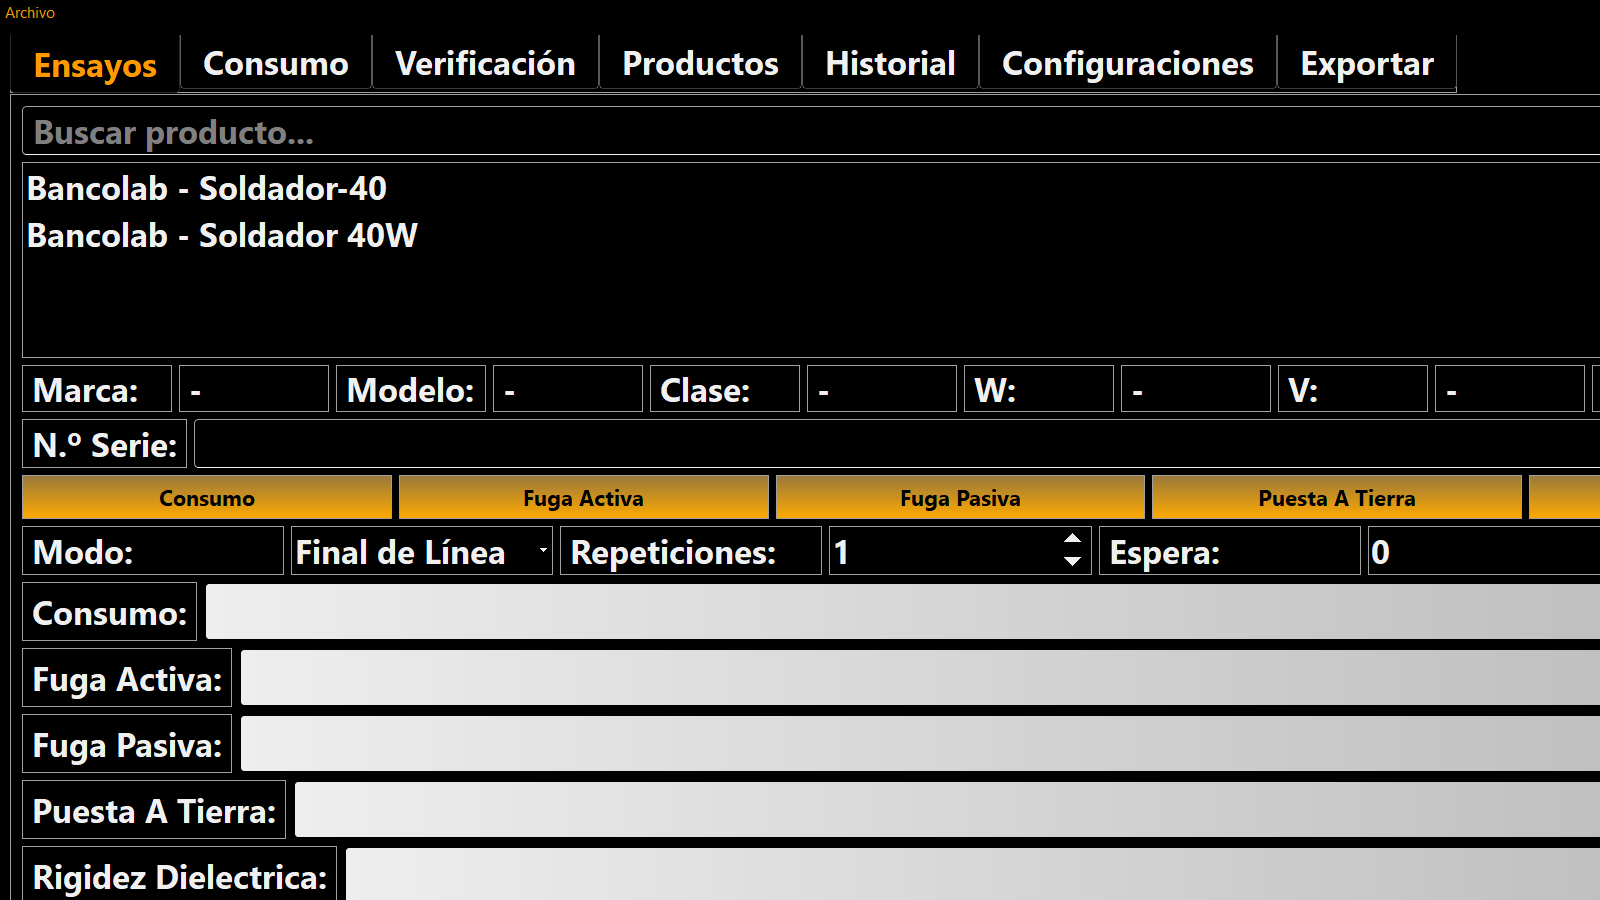
\includegraphics[width=\linewidth]{gui_ensayos.png}
        \caption{Ensayos.}
    \end{subfigure}\hfill
    \begin{subfigure}[b]{0.49\linewidth}
        \centering
        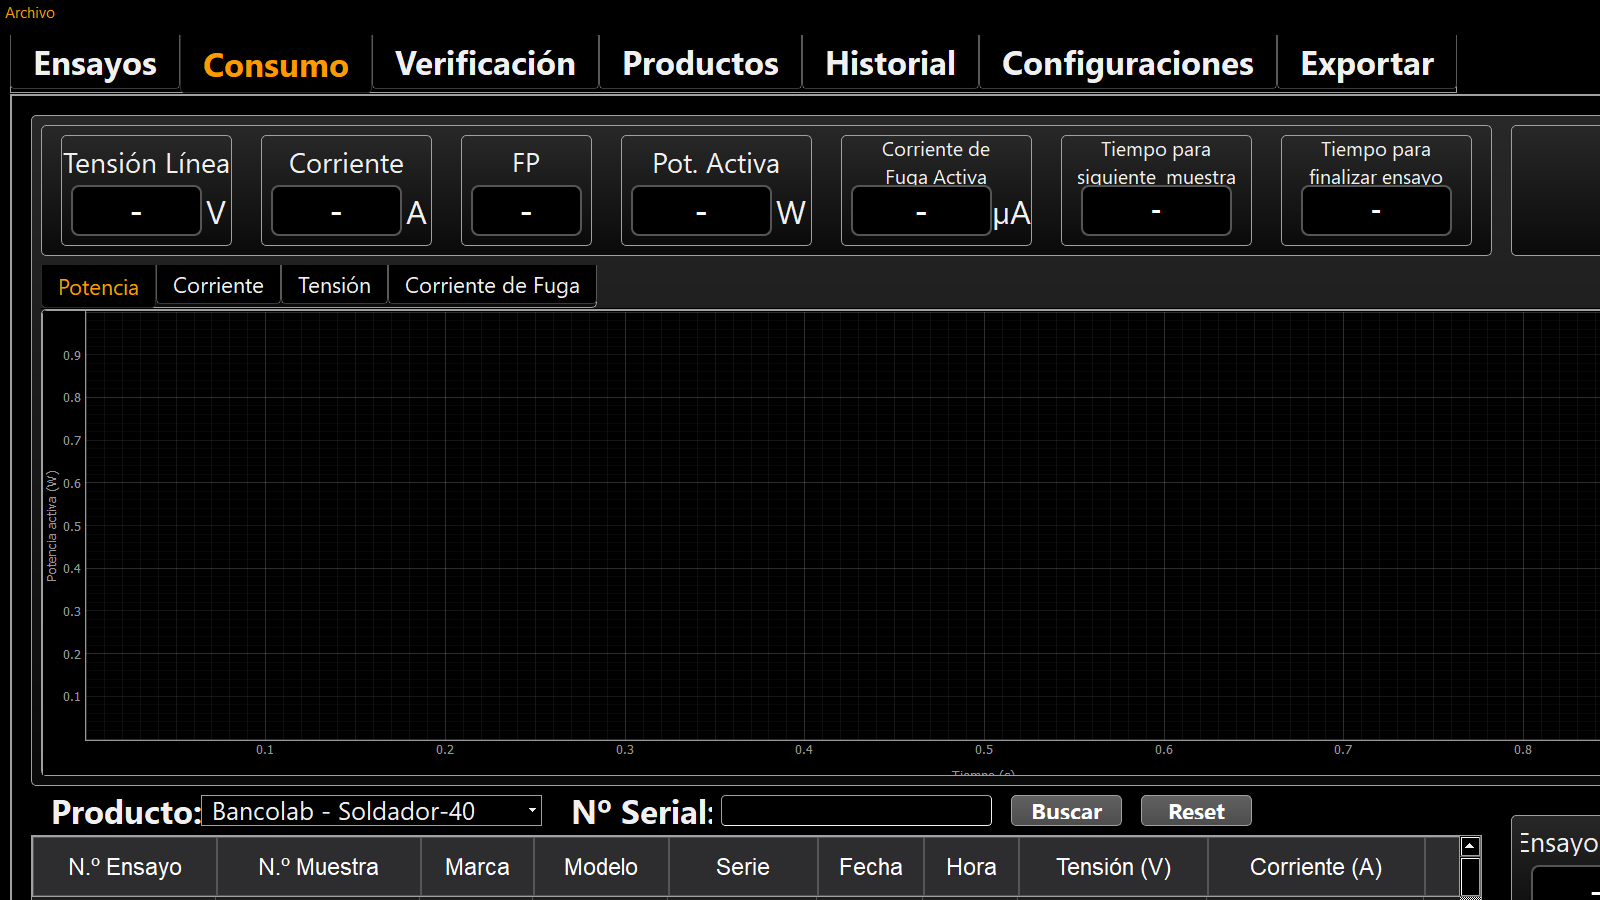
\includegraphics[width=\linewidth]{gui_consumo.png}
        \caption{Consumo.}
    \end{subfigure}\\[1em]
    \begin{subfigure}[b]{0.49\linewidth}
        \centering
        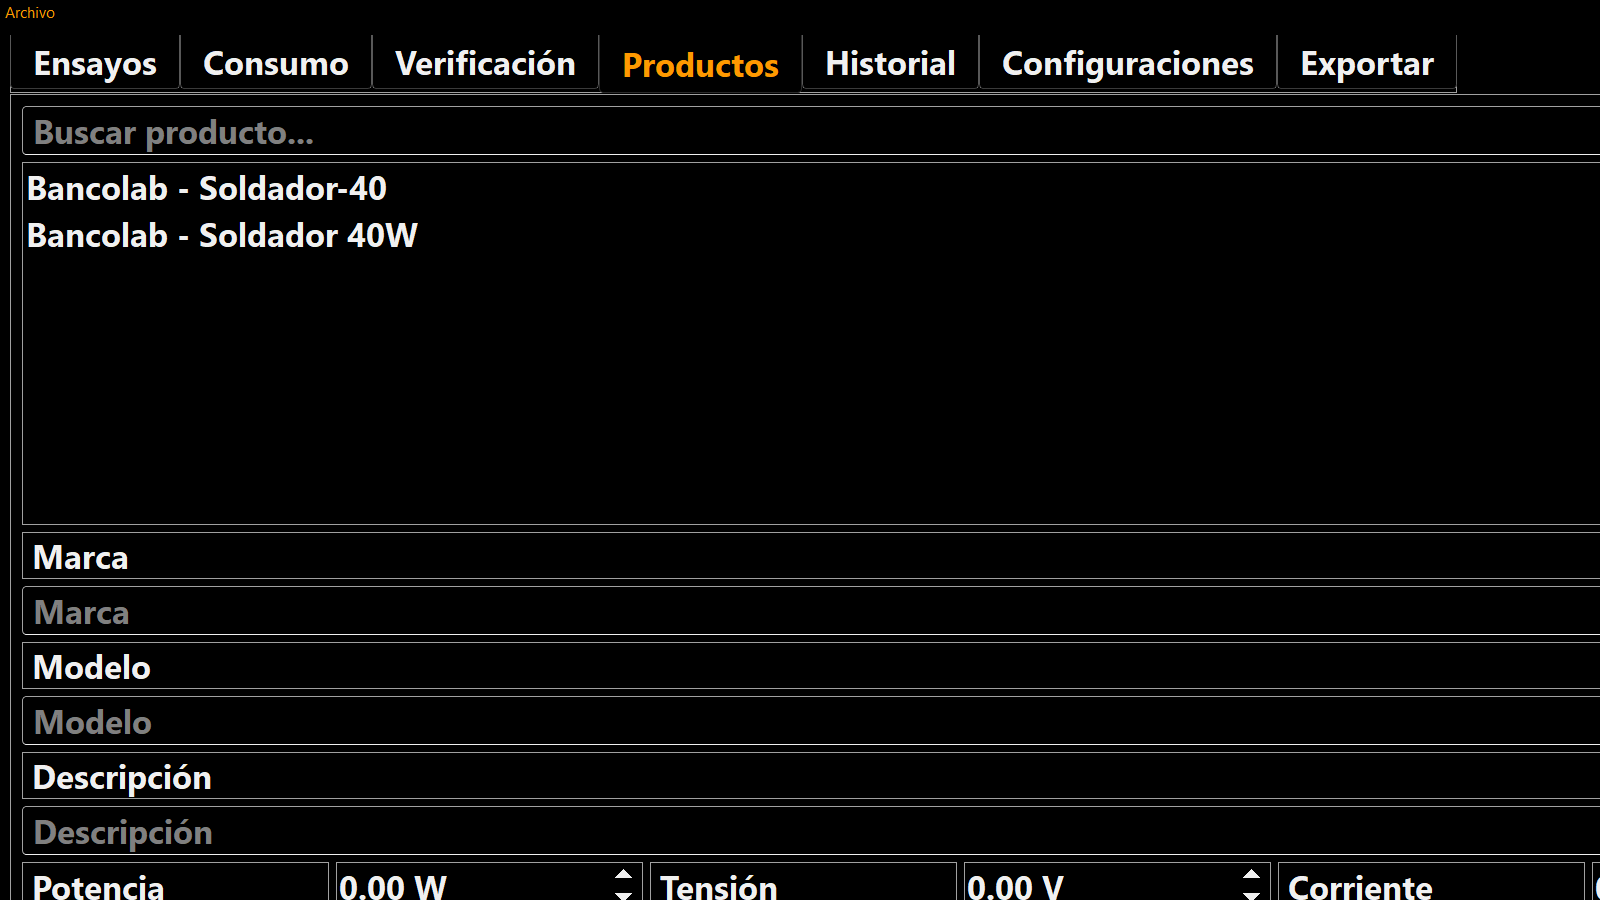
\includegraphics[width=\linewidth]{gui_productos.png}
        \caption{Productos.}
    \end{subfigure}\hfill
    \begin{subfigure}[b]{0.49\linewidth}
        \centering
        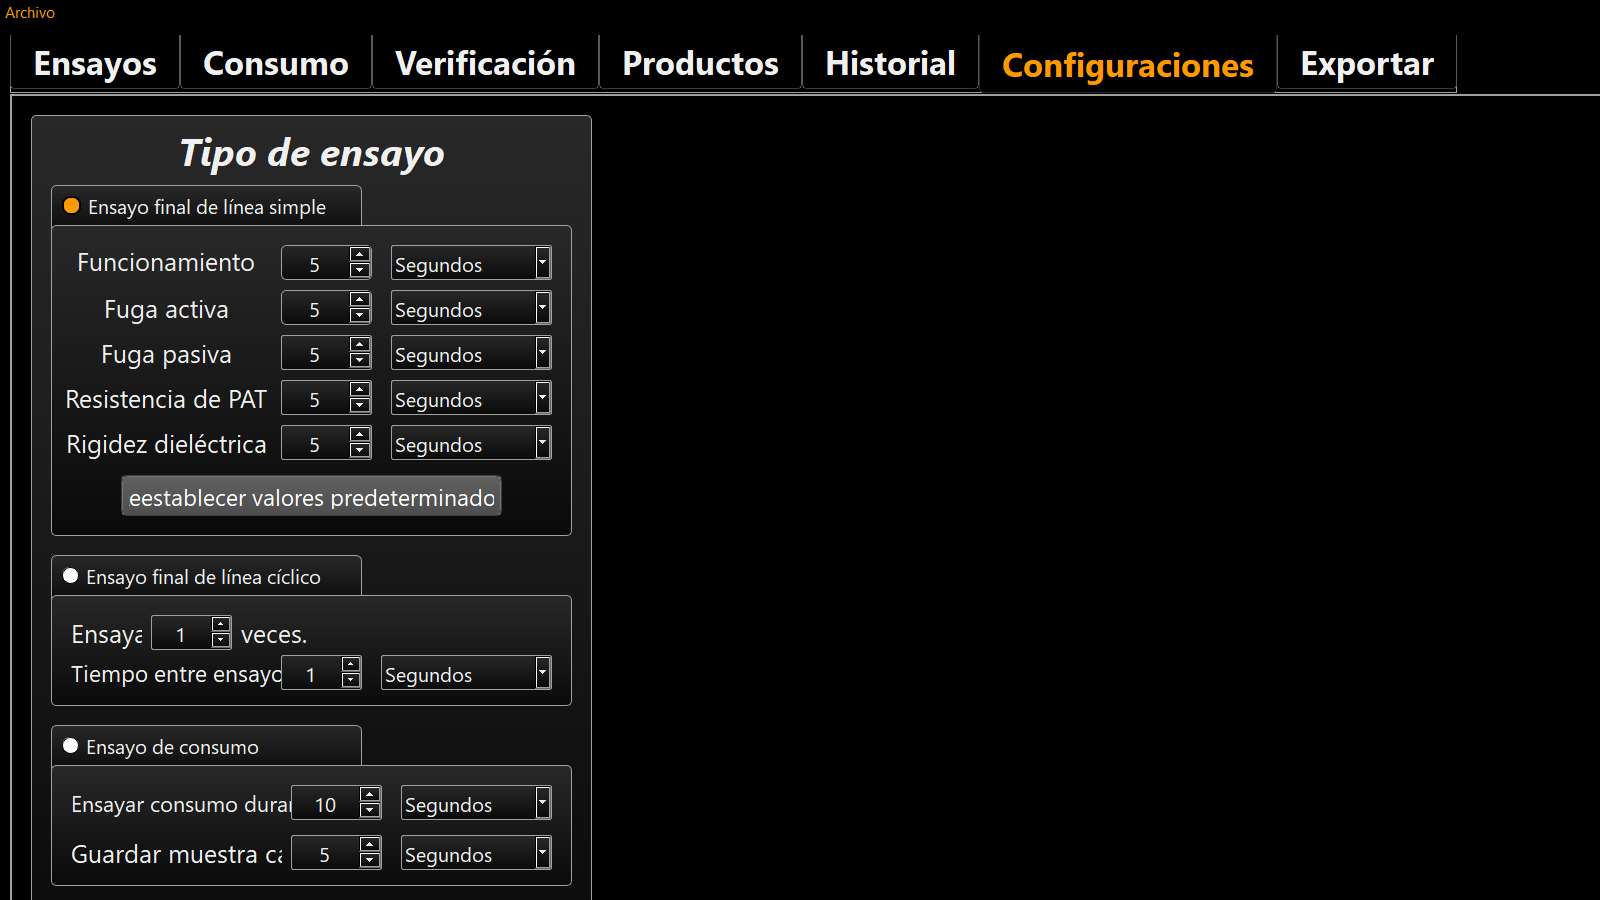
\includegraphics[width=\linewidth]{gui_configuraciones.png}
        \caption{Configuraciones.}
    \end{subfigure}
    \caption{Pantallas principales de la interfaz gráfica.}
    \label{fig:gui}
\end{figure}

% ------------------------------------------------------------
\subsection{Criterios metodológicos de los ensayos}
\label{subsec:criterios_ensayo}
% ------------------------------------------------------------

\begin{itemize}
    \item \textbf{Ensayos de rutina:} por ser un equipo de final de línea, se
          aplican los ensayos de rutina del Anexo~A (rigidez dieléctrica y
          puesta a tierra); para fuga y consumo, que el Anexo~A no contempla, se
          toman los límites de las cláusulas~13, 16 y~10.
    \item \textbf{Peor caso frente a promedio:} en rigidez dieléctrica y puesta a
          tierra el veredicto se toma sobre el peor valor del intervalo (tensión
          mínima y corriente máxima, o resistencia máxima), porque una sola lectura
          fuera de límite indica una falla de seguridad. En consumo se usa el
          promedio del intervalo, que representa la potencia en régimen.
    \item \textbf{Condiciones de validez:} si la tensión de rigidez no alcanzó el
          valor de ensayo, o si la corriente de puesta a tierra no llegó a
          \SI{10}{\ampere}, el aislamiento o la continuidad no se verificaron en
          condiciones de norma y el resultado es FALLA.
    \item \textbf{Estabilización:} en consumo se descartan las lecturas tomadas
          mientras el contactor cierra y el medidor se actualiza (dos lecturas en
          el ensayo de final de línea y \SI{3}{\second} en el perfil de consumo).
    \item \textbf{Falla segura:} en los ensayos de seguridad, una lectura fallida
          del medidor produce FALLA y nunca un aprobado; ante cualquier error, el
          software abre los relés y el contactor.
\end{itemize}

% ------------------------------------------------------------
\subsection{Procedimiento de pruebas}
\label{subsec:procedimiento_pruebas}
% ------------------------------------------------------------

\begin{itemize}
    \item \textbf{Pruebas unitarias:} cada componente del software se valida de
          forma independiente, con el hardware simulado.
    \item \textbf{Pruebas de integración:} se evalúa la interacción entre módulos,
          desde la adquisición hasta el almacenamiento y la interfaz, incluida la
          ventana principal en modo sin pantalla.
    \item \textbf{Pruebas en banco:} se opera la aplicación real con el hardware
          real sobre cargas conocidas (una resistiva y una con motor), registrando
          los resultados en una base de datos separada.
\end{itemize}
